\newpage
\section{Integration (bi-variat)}
Als bi-variate Integrale versteht man Integrale, die siech über zwei unabhängige Variablen erstrecken.
Sie haben die Form
\[
    \int\limits_{\Omega} f(\omega)\cdot \diff \omega =\int\limits_{X} \int\limits_{Y} f(x;y) \cdot dy \cdot dx
\]
wobei $ \Omega \subset \mathbb{R}^2 $, $ X \subset \mathbb{R} $ und $ Y \subset \mathbb{R} $ ist.

\subsection{Normalbereich}

TODO: WTF ist ein Normalbereich?
Schnitte sind Strecken (Intervalle) für x, y, ...

\subsection{Zweidimensionale Koordinatensysteme}
Neben den Kartesischen Koordinatensystemen kommen in zweidimensionalen Räumen auch Polare Koordinatensysteme zum einsatz.
Die beiden Systeme können mit Hilfe der Trigonometrie in einander überführt werden.

\subsubsection{Umrechnung Kartesisch $\leftrightarrow$ Polar}
\begin{minipage}{0.29\linewidth}
    \myul{Polar zu Kartesisch}
    \[
    \begin{pmatrix}
        x \\
        y
    \end{pmatrix}
    =
    \begin{pmatrix}
        r * \cos{\phi}\\
        r * \sin{\phi}
    \end{pmatrix}
    \]
\end{minipage}
\hfill
\begin{minipage}{0.29\linewidth}
    \myul{Kartesisch zu Polar}
    \[
    \begin{pmatrix}
        r \\
        \phi
    \end{pmatrix}
    =
    \begin{pmatrix}
        \sqrt{x^2+y^2}\\
        \tan^{-1}{\frac{y}{x}}
    \end{pmatrix}
    \]
\end{minipage}
\hfill
\begin{minipage}{0.29\linewidth}
    \begin{center}
        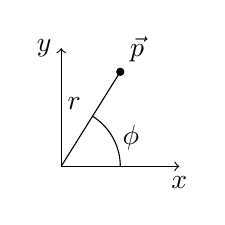
\begin{tikzpicture} [scale = 1.5]
            % Kartesische Achsen
            \draw[->] (0, 0) -- (1, 0) node [below] {$x$} ;
            \draw[->] (0, 0) -- (0, 1) node [left]  {$y$} ;

            % Punkt p
            \fill (0.5, 0.8) circle (1pt) node [anchor=south west] {$\vec{p}$};

            % Länge r
            \draw (0, 0) -- (0.5, 0.8) node [midway, above left] {$r$};
            % Winkel phi
            \draw (0.5, 0) arc (0:58:0.5) node [midway, right] {$\phi$};
        \end{tikzpicture}
    \end{center}
\end{minipage}

Dabei ist zu beachten, dass $\tan^{-1}$ nur werte von $-180\degree$ bis $180\degree$ liefert. 
$\phi$ wird also, je nach dem in welchem Quadranten sich $\vec{p}$ befindet, nach folgendem Schema berechnet:
\begin{center}
    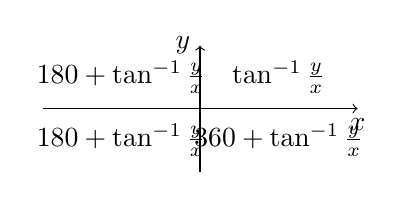
\begin{tikzpicture}
        % Achsen 
        \draw [->] (-2, 0) -- (2, 0) node [below] {$x$};
        \draw [->] (0, -0.8) -- (0, 0.8) node [left] {$y$};
        % Formeln
        \node at ( 1,  0.4) {$\tan^{-1}\frac{y}{x}$};
        \node at ( 1, -0.4) {$360\degree + \tan^{-1}\frac{y}{x}$};
        \node at (-1, -0.4) {$180\degree + \tan^{-1}\frac{y}{x}$};
        \node at (-1,  0.4) {$180\degree + \tan^{-1}\frac{y}{x}$};
    \end{tikzpicture}
\end{center}

Um eine ganzes Integral vom einen Koordinatensystem ins andere zu überführen, muss zum einen die Funktion $ f(x, y) $ zu $ f(r, \phi) $ (oder umgekehrt) umgeschrieben, sowie die differentiale angepasst werden.
Hier dafür einige gängige Elemente:

\begin{tabular}{l c c}
                         & \bf{Kartesisch}                   & \bf{Polar}                                                     \\
    \bf{x-Achsenelement} & $\diff x$                         & $\diff x = \cos \phi \diff r - r \sin \phi \diff \phi$    \\
    \bf{y-Achsenelement} & $\diff y$                         & $\diff x = \sin \phi \diff r + r \cos \phi \diff \phi$    \\
    \bf{Linienelement  } & $\diff s^2 = \diff x^2 \diff y^2$ & $\diff s^2 = \diff r^2 + r^2 \diff \phi^2$                \\
    \bf{Flächenelement } & $\diff A = \diff x \diff y$       & $\diff A = r \diff r \diff \phi$                          \\
\end{tabular}

\subsection{2D Transformation Polar zu Kartesisch}
TODO: Das isch ja ds gliiche wie obe beschribe, oder?
      Wänn da no meh ane sött wüsstich nöd was... -Flurin
T $=$ Transformation
\[
    \text{Polar } (r,\phi) \xrightarrow{T} (x,y) \text{ Kartesisch}
\]

\[
\begin{pmatrix}
    x=r\cdot\cos(\varphi) \text{ } \cor{\mathbb{R}} \\
    y=r\cdot\sin(\varphi) \text{ } \cor{\mathbb{R}} 
\end{pmatrix}
\text{2D}
\]

Die Funktionen für $x$ und $y$ sind skalare Funktion.

    \begin{ctabular}{ll}
        $x=x(r;\varphi)$ & $ y=y(r;\varphi)$
    \end{ctabular}

\subsection{Derivative, Ableitung}
TODO: Idk was da ane söll -Flurin

\subsection{3D Volumenberechnung}
TODO: Wie will me i 2D Volumen berächne?! -Flurin

$$V=\int_{x_{\min}}^{x_{\max}} \left[\int_{y_{\min}(x)}^{y_{\max}(x)} f\left(x;y\right)  \,dy \right] \,dx $$
